\section{Thickness of the target layers} 
Most of the particles pass directly through the target without scattering. However, a small amount do scatter. When particles pass through the first layer they loose energy. As a consequence, there will be a difference in the energy of the particles entering the first and the second layer. 

By comparing measurements of scattering on the target with gold layer facing the beam and the carbon layer facing the beam, the distributions for scattering on carbon and gold are observed at different energies \cref{fig_sketch_thickness}. 

\begin{figure}[h]
\centering
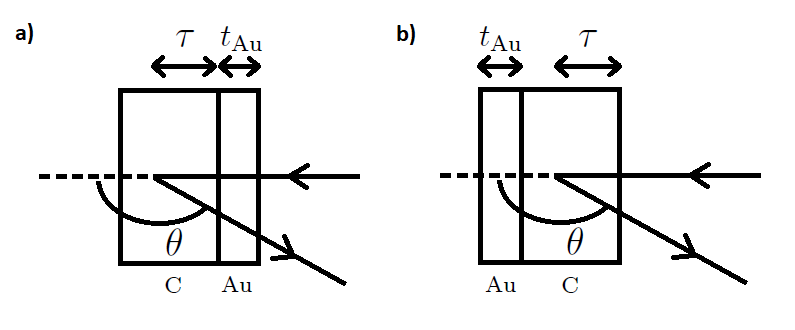
\includegraphics[width=0.99\columnwidth]{tykkelse.png}
\caption{Sketch of how to determine thickness of the target carbon layer from the energy difference between: a) gold layer facing the beam and b) carbon layer facing the beam.}
\label{fig_sketch_thickness}
\end{figure}


%The energies of the scattered protons is due to the ratio between the mass of the protons and the mass of the target. 
The energy differences are proportional to the thickness of target layers. To determine the thickness of the carbon layer we consider what happens to the energy in the two following situations. In situation a) gold is facing the beam, and the final energy $E_{f,a}$ is given as the incoming energy $E_i$ minus the energy lost due to scattering on gold:
\begin{equation}
E_{f,a} = E_i (1-f_\mathrm{Au}(\theta)), 
\end{equation}
where $f_{Au}$ is the function giving the relation between the incoming energy and the particle energy after scattering on gold in equation (6).
In situation b) carbon is facing the beam, and the final energy is given as the incoming energy minus the energy lost due to the particles; passing through the carbon layer, scattering on gold, and passing through the carbon layer again on the way out. 
\begin{align}
E_{f,b} &= E_i - t_\mathrm{C} \left(\frac{dE}{dx}\right)_\mathrm{C} \nonumber
\\ &- f_\mathrm{Au}(\theta) \left(E_i - t_\mathrm{C} \left(\frac{dE}{dx}\right)_\mathrm{C} \right)\nonumber 
\\ &- \frac{t_\mathrm{C}}{\cos(\pi-\theta)} \left(\frac{dE}{dx}\right)_\mathrm{C},
\end{align}
where $t_\mathrm{C}$ is the thickness of the carbon layer and
$\left(\frac{dE}{dx}\right)_\mathrm{C}$ is the stopping power of carbon. The
stopping power of carbon and gold are found to be $8.5$ and $34 \;
\si{\electronvolt}/(10^{15}$ atoms/$\si{\centi\metre}^2$), respectively. The
values were read off a table next to the laboratory computer.

The energy difference for the peak position for gold is found as the difference
between the two situations, $\Delta E_\mathrm{Au} = E_{f,a} - E_{f,b}$. Thus,
the thickness of the carbon layer is found as
\begin{equation}
t_\mathrm{C} = \frac{\Delta E_{\mathrm{Au}}}{\left(\frac{dE}{dx}\right)_\mathrm{C} \left(1 - f_\mathrm{Au}(\theta) - \frac{1}{\cos(\theta)} \right)}
\end{equation}


The thickness of the gold layer is found using the same approach. 

\begin{table}[h]
\centering
\caption{Thickness of the target layers determined from change in energy.}
\begin{tabular}{CC}
\toprule
\multicolumn{2}{c}{Target layer thickness}\\
\midrule
\mathrm{C} & 2325 \pm 51 \; \AA \\
\mathrm{Au} & 262 \pm 26 \; \AA \\
\bottomrule
\end{tabular}

\label{tab_thickness}
\end{table}

%\begin{equation}
%\Delta E_{Au} = t_C \left(\frac{dE}{dx}\right)_C \left(1 - f_E(\theta) + %\frac{1}{\cos(\pi-\theta)} \right),
%\end{equation}



\begin{figure}[t]
\centering
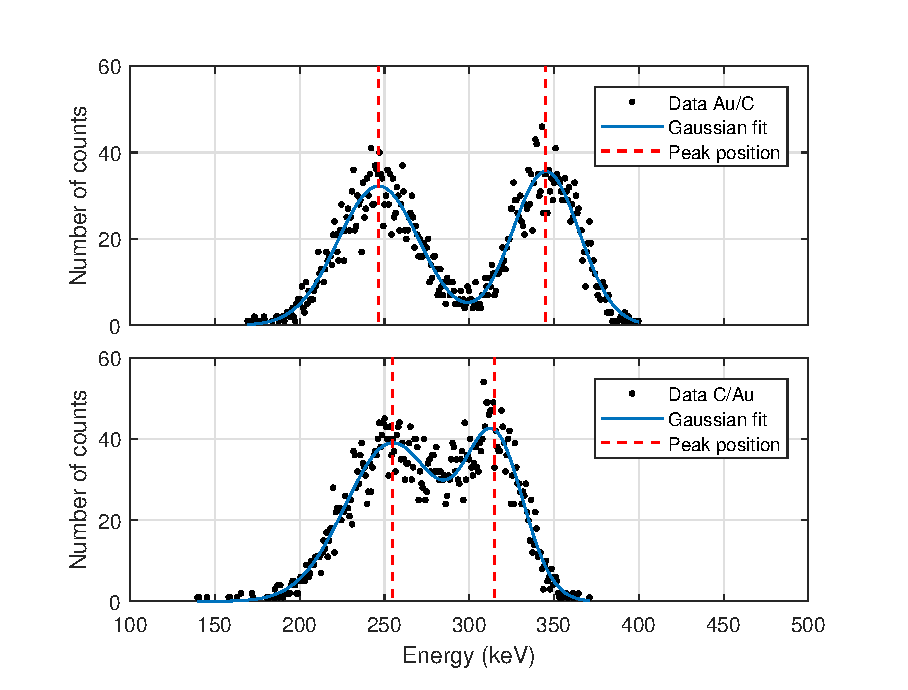
\includegraphics[width=0.99\columnwidth]{Dterminethicknessplot.eps}
\caption{Thickness of target layers determined from change in energy. Upper: gold layer facing the beam. Lower: carbon layer facing the beam.}
\label{fig_thickness}
\end{figure}

The scattering angle for thickness determination was chosen such that the distributions overlap as little as possible while still having sufficient number of counts for the case of gold facing the beam. However, significant overlap of the distributions is observed when turning the target 180 $\si{degrees}$ to situation b) where the carbon layer faces the beam. As discussed previously, overlap of distributions as well as low number of counts makes fitting two Gaussian functions difficult and thus affects the uncertainties for the determined fitting parameters.  In addition, the energy change for the carbon peak is very small, which complicates the determination of the precise thickness of the gold layer.








